\todo[inline]{
\textbf{Todo}

- a problem or phenomenon you want to study

- the reasoning behind your choice of topic (gap in knowledge)

- the research question or hypothesis you set out to investigate
}
\section{Teleoperation}

\todo[inline]{
\textbf{Todo}

- explain why focus will be on manoeuvring robots
}

Teleoperation of robots will become more and more common as the technology makes it possible for people to accomplish tasks in remote, inaccessible and hostile environments. The range of applications are long, space exploration, military missions, undersea operations and surgery are some of them.

Unmanned vehicles comes in a variety of configurations and can be divided into unmanned aerial vehicles (UAV), ground (UGV), underwater (UUV) where the latter is also sometimes referred to as a remotely operated vehicle (ROV).

Because of the nature of teleoperation the situational awareness and telepresence is compromised because of numerous factors. In a teleoperation controlled through video feed some of the influencing factors could be time latency, frame rates, missing frame of reference, two-dimensional views, field of view and more.

\citep{Fong2001} "With manual control, performance is limited by the operator's motor skills and his ability to maintain situational awareness."

\citep{Chen2007} went through more than 150 papers checked different teleoperation factors and how they influence user performance.

"Arthur et al. [89] also found latency (ranging from 50 to 550 ms) to be a more important factor than FR (30, 15, or 10 fps) for their participants 3-D tracing task performance."

\section{Video latency and user performance}

\citep{Chen2007}

"people are generally able to detect latency as low as $10-20$ ms [83]. Generally, when system latency is over about 1 s, the operators begin to switch their control strategy to a "move and wait" "

"Studies have also shown that high latency lags tend to re-
duce perceived telepresence"

"Woods et al. [16] suggested that achieving functional presence might be a more realistic goal for teleoperation user interface design. Functional presence occurs when the teleoperator receives sufficient perceptual cues to effectively conduct teleoperations"

"For example, time delays as short as 170 ms affected driving performance. If these delays cannot be engineered out of the system, it is suggested that predictive displays or other decision support be provided to the operator."

\citep{Appelqvist2007} "Because of the teleoperation delay, human drivers
tend to cause the vehicle to oscillate with their "correcting" steering commands" 

Time delay present a problem since the user has to remember what has already been done, and this does not match with the image they are seeing.

\citep{Ricks2004} " The mental load required to keep track of robot pose and compensate for delay adversely affects the operator's ability to effectively control the robot."

"There are many reasons to study teleoperation, espe-
cially from the standpoint of improving the user interface. Teleoperation can be the most effective way to control mobile robots because it is easy to implement and easy for people to understand. Teleoperation is also a very simple autonomy level that allows us to study the interface itself apart from the intelligence derived from autonomy."

\subsection{Reduce detrimental effects of video latency}
\todo[inline]{
\textbf{Todo}

- can be divided into how the tools, camera and environment move with respect to each other

- mesh generation

- phantom robot

- Autonomy

- AR with predicted future 3D geometry

- Having stored local bigger images on cropping that image

- capturing 3d data from scene and predicting the movement in that scene

- displaying a generated 3d scene from remote images

- egocentric vs ecocentric
}

There are many ways to mitigate the effects of teleoperation with video latency. By increasing the level of autonomy the operator would have to give less commands. A fully autonomous setup would require no user input and the negative effects of time delay would be completely eliminated.

\citep{Goodrich2001} Made a comparison between neglect and time delay and argued that adjustable autonomy could be used to increase the robot effectiveness. And also mentions that a more autonomous robot is required when longer time delays are present. On the other side he also mentiones that "as autonomy level increases, the breadth of tasks that can be handled by a robot decreases."

In some cases, autonomy is essential to accommodate for communication delays. \citep{Dorais1999}

The second possibility is to introduce predictor displays with phantom robots. In this setup the future behaviour of the robot is predicted from user input and the last know configuration of the robot. This is then shown as computer generated version, or phantom robot in real-time.

\citep{Chen2007} "Based on this and other experimental results, Sheridan [86] recommended that supervisory control and predictor displays be used to ameliorate the negative impact of time delays on teleoperation."

"predictive displays have been shown to be able to reduce task performance time by 50\%-150\% [68]"

The third option is present more information to the operator so that he or she has a better foundation to understand how user input would impact the future state of the robot. This could include showing graphs of the last inputs, or giving feedback when the user does something.

\citep{Miller2005} performed a test where they "Instead of predicting where the rover will be, we remind the operator of what they have told the rover to do by providing them with a streaming command indicator."


\section{Predictive displays}

Predictive displays will predict the future configuration based on user input and show real-time predicted configuration.

Predictive displays can be used in conjugating with augmented reality (AR) or virtual reality (VR). The drawback with VR is that it requires extensive information about the remote location and computer knowledge and power because the location with the robot has the be reconstructed digitally. This is often used in cases where industrial robots are used. Here each of the joints and surrounding area can be precisely calculated. Telerobotic servicing with robotic arms with overlayed 3D grapical robots \citep{Kim1993}

\citep{Ricks2004} tested a predictive display based with a phantom robot seen from a tethered perspective is placed together with the video feed in AR fashion, \figref{figRicks2004}. This required a laser range finder to model the environment. The prediction were performed by using the known position and velocity of the robot and calculating the predicted position and orientation based on user input.

Another approach is by combining visual tracking and image-based 3d rendering, creating a computer generated world and extrapolating what the camera would see next after it has gotten the current user commands. \citep{Hu2015} did this, but as they mentioned this relatively required smooth motion and advanced model generation algorithms.

Another way producing predictive displays is by recording 360 degrees video on a low frame rate and only displaying a smaller selection of this to the user. When the the camera or robot is moved the predicted section can be displayed immediately by moving the selection in that direction. \citep{Baldwin1999}

\begin{figure}[h!]
    \centering
    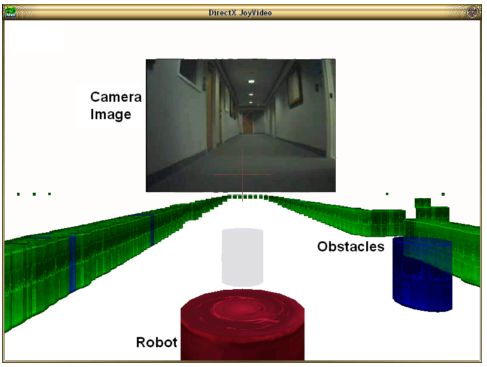
\includegraphics[width=.7\textwidth]{ricks2004display}
    \caption{Predictive display \citep{Ricks2004}}
    \label{figRicks2004}
\end{figure}

\begin{figure}[h!]
    \centering
    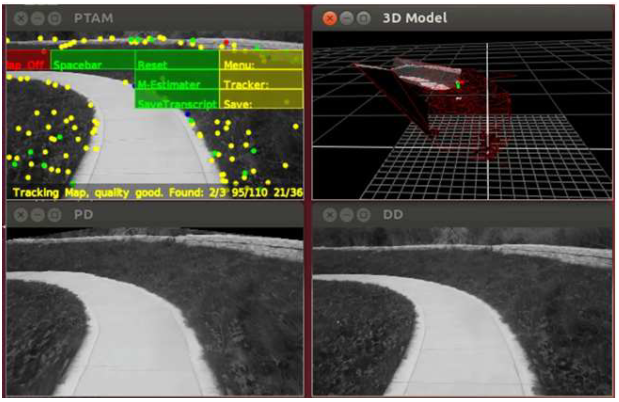
\includegraphics[width=.7\textwidth]{hu2015display}
    \caption{Predictive display \citep{Hu2015}}
\end{figure}

\section{Problem statement}

\section{Engage eduROV project}